\documentclass[10pt,a4paper,notitlepage]{article}
\usepackage[utf8]{inputenc}
\usepackage[english]{babel}
\usepackage{amsmath}
\usepackage{amsfonts}
\usepackage{amssymb}
\usepackage{graphicx}
	\graphicspath{ {Images/eps/} }


\usepackage[left=2cm,right=2cm,top=2cm,bottom=2cm]{geometry}
\begin{document}
\section{HGT scenarios: four species and five genes}	

\subsection{Possible scenarios}


\subsection{Colored proteinortho graphs}
%L_T is the gene set. Define the sets S_1 and S_2 
In each proteinorto graph, draw with color (not black) an edge $e$ iff it is directed to/from the donor ($h$) or an HGT ($h', h'',...$) of the HGT, i.e, 
		\begin{center}
			 $e=(h,x),e=(x,h),e=(h',x)$ or $e=(x,h')$, $\forall x\in L_T$\\
		\end{center}

We will \textit{add} the two colored graphs by ovelaping them. The result will be a five-vertex graph, the \textit{colored proteinortho graph}.
% Example:


\subsection{Coloring the scenarios}
	\subsubsection{Scenarios for $T_1$}


	\subsubsection{Scenarios for $T_2$}		
	\begin{tabular}[h]{|c|}
		\hline	
		Scenario 
		$\;\;\;\;\;\;\;\;\;\;\;\;\;\;\;\;\;\;\;\;\;\;\;\;\;\;\;\;\;\;\;\;\;\;\;\;\;\;\;\;\;\;\;\; {G}_1$
		$\;\;\;\;\;\;\;\;\;\;\;\;\;\;\;\;\;\;\;\;\;\;\;\;\;\;\;\;\;\;\;\;\; {G}_2$ 
		$\;\;\;\;\;\;\;\;\;\;\;\;\;\;\;\;\;\;\;\;\;\;\;\;\;\;\; {G}_1 \times {G}_2  \;\;\;\;\;\;\;\;\;\;\;\;$\\		
		\hline
	\end{tabular}
	\\
\begin{enumerate}
\item 
		
\includegraphics[scale=0.7]{Images/eps/fig1}\\
\item
		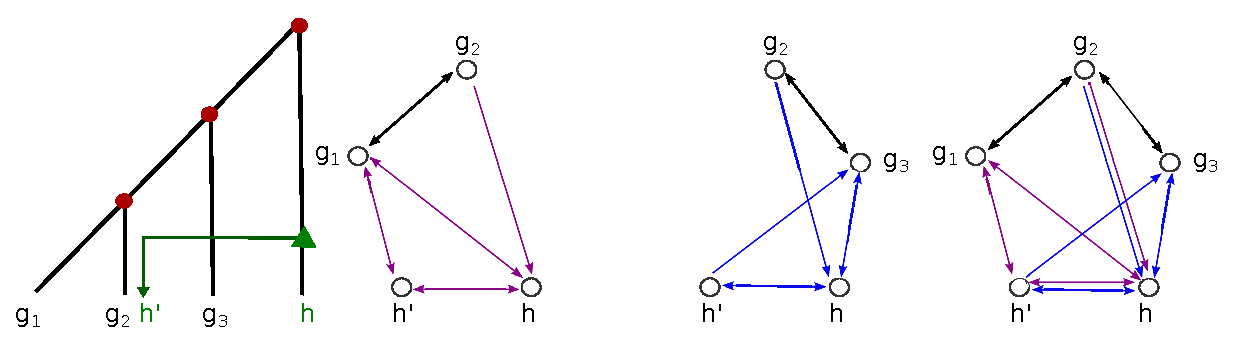
\includegraphics[scale=0.7]{Images/eps/fig2}\\
\item
		
\includegraphics[scale=0.7]{Images/eps/fig3}\\
\item
		
\includegraphics[scale=0.7]{Images/eps/fig4}\\
\item
		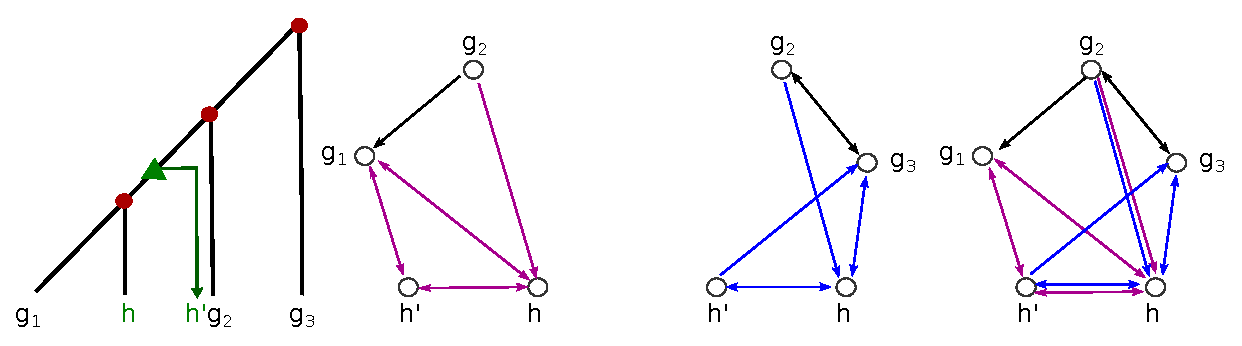
\includegraphics[scale=0.7]{Images/eps/fig5}\\
\item
		
\includegraphics[scale=0.7]{Images/eps/fig6}\\
\item
		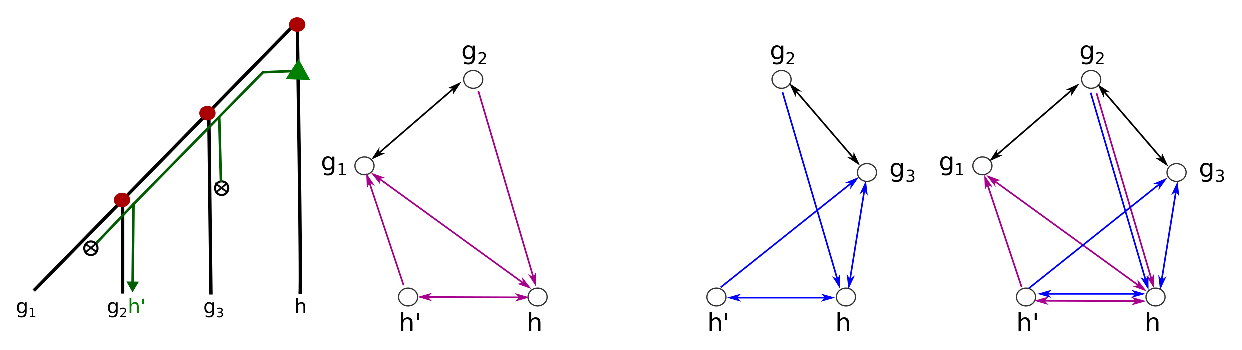
\includegraphics[scale=0.7]{Images/eps/fig7} \\
\item
		
\includegraphics[scale=0.7]{Images/eps/fig8} \\

\end{enumerate}

%	\includegraphics[scale=0.7]{fig11} \\

	
\subsection{How to identify HGT and correct the orthology graph}
	Let T be a tree with $L_T=\{ g_1, g_2, g_3, g_4, h\}$ which correspond to four species $A, B, C$ and $D$, and say that $g_1$ and $g_2$ are in the same species, implying that one of them was acquired via HGT. We assume it is known which gene is the HGT donor ($h$). 
	\\
	How to correct the orthology graph of T:
	\begin{enumerate}
		\item Identify the HGT receptor ($h'$):
			\begin{itemize}
				\item Let $G_1$ and $G_2$ be the sets of four genes such that $\{g_1, g_2, h\} \in G_1,G_2$.
				\item Generate the colored proteinortho graphs for $G_1$ and $G_2$ and add them to generate a five-vertex graph with two colors.
				\item Identify the bidirectional edges of $g_1$ and $g_2$.
				\item Choose as $h'$, the vertex ($g_1$ or  $g_2$) which has a bicolored and bidirectional edge.
%				\item \textit{Choose as $h$ the other vertex of this bi-colored and bidirectional edge.}
			\end{itemize}
		\item Delete $h'$ and its edges from the five-vertex graph.
		\item Complete the unidirectional edges to bidirectional edges. 
	\end{enumerate}
	
\end{document}